\pdfbookmark{Общая характеристика работы}{characteristic}             % Закладка pdf
\section*{Общая характеристика работы}
\newcommand{\actuality}{\pdfbookmark[1]{Актуальность и разработанность темы}{actuality}\underline{\textbf{\actualityTXT}}}
%\newcommand{\progress}{\pdfbookmark[1]{Разработанность темы}{progress}\underline{\textbf{\progressTXT}}}
\newcommand{\aim}{\pdfbookmark[1]{Цели}{aim}\underline{{\textbf\aimTXT}}}
\newcommand{\tasks}{\pdfbookmark[1]{Задачи}{tasks}\underline{\textbf{\tasksTXT}}}
\newcommand{\aimtasks}{\pdfbookmark[1]{Цели и задачи}{aimtasks}\aimtasksTXT}
\newcommand{\novelty}{\pdfbookmark[1]{Научная новизна}{novelty}\underline{\textbf{\noveltyTXT}}}
\newcommand{\influence}{\pdfbookmark[1]{Практическая значимость}{influence}\underline{\textbf{\influenceTXT}}}
%\newcommand{\methods}{\pdfbookmark[1]{Методология и методы исследования}{methods}\underline{\textbf{\methodsTXT}}}
\newcommand{\defpositions}{\pdfbookmark[1]{Положения, выносимые на защиту}{defpositions}\underline{\textbf{\defpositionsTXT}}}
\newcommand{\reliability}{\pdfbookmark[1]{Достоверность}{reliability}\underline{\textbf{\reliabilityTXT}}}
%\newcommand{\probation}{\pdfbookmark[1]{Апробация}{probation}\underline{\textbf{\probationTXT}}}
\newcommand{\contribution}{\pdfbookmark[1]{Личный вклад}{contribution}\underline{\textbf{\contributionTXT}}}
\newcommand{\publications}{\pdfbookmark[1]{Публикации}{publications}\underline{\textbf{\publicationsTXT}}}


{\actuality} Геном прокариот представляет собой сложно организованную структуру. Помимо кодирующих и регуляторных областей, в нем имеется ряд элементов, необходимых для взаимодействия ДНК с молекулярными комплексами, осуществляющими процессы транскрипции, репликации и репарации. Пространственная укладка генетического материала в клетке не случайна и выполняет ряд регуляторных функций. Подобные наблюдения меняют представление о геноме, как о простом хранилище последовательностей генов расположенных в случайном порядке, и позволяют говорить об архитектуре генома --- закономерностях, которые необходимы для успешного функционирования живой клетки.

К настоящему времени известен ряд элементов геномной организации. Гены, продукты которых необходимы клетке в больших количествах, расположены рядом с сайтом начала репликации, поскольку в быстро делящихся клетках такое расположение позволяет повысить уровень их экспрессии за счет увеличения копийности матричной ДНК. Пространственная укладка ДНК может сближать гены, расположенные в разных областях линейной последовательности, что оказывается полезно для генов, кодирующих регулятор и его мишени. Экспериментально было установлено, что действие глобальных регуляторов, таких как гистоноподобный белок H-NS, зависит от местоположения генов мишеней. Склонность к транскрипции (уровень экспрессии генов, не зависящий от их последовательности) значительно меняется в зависимости от положения гена в хромосоме. Взаимодействие РНК-полимераз, возникающее за счет изменения уровня суперскрученности ДНК, может играть роль в регуляции транскрипции соседних генов.

Геномные перестройки и горизонтальный перенос генов могут приводить к изменению оптимального расположения генов и других элементов генома, что может приводить к снижению жизнеспособности организма. Известно, что изменения в геномах преимущественно локализуются в отдельных местах --- "горячих"\ точках. Возможно, эти участки свободны от "архитектурных"\ ограничений, и таким образом более толерантны к изменениям. Возможно, эти участки имеют некоторые признаки, способствующие более высокой частоте происходящих изменений. Нельзя исключить возможность, что ``горячие'' точки возникли в результате генетического дрейфа а их расположение случайно и не обладает функциональным значением. Какие из этих вариантов, и в какой степени, реализуются в действительности, к настоящему моменту, неизвестно: локализация "тихих"\ консервативных участков и "горячих"\ высокоизменчивых областей не имеет общепринятых объяснений. Для проведения исследований в данной области необходим инструмент, позволяющий находить и анализировать области генома с повышенной и пониженной изменчивостью. Разработка и применение подобного инструментария и стала основной темой данной работы. 

{\aim} данной работы является разработка программного конвейера для выявления высокоизменчивых областей геномов прокариот и применение его для анализа изменчивости в локусах генома \textit{Escherichia coli}, ассоциированных с болезнью Крона.


Для~достижения поставленной цели необходимо было решить следующие {\tasks}:
\begin{enumerate}[beginpenalty=10000] 
  \item Разработать алгоритм оценки уровня изменчивости геномов, основанный на их графавом представлении.
  \item Сравнить профили изменчивости геномов принадлежащих различным родам, видам и подвидовым структурам прокариот.
  \item Оценить вклад различных факторов геномной организации в уровень изменчивости генома. 
  \item Разработать алгоритм визуализации подграфов, соответствующих отдельным локусам генома.
  \item Разработать алгоритм поиска и выявить в геноме \textit{E. coli} опероны, которые значимо чаще встречаются в изолятах от пациентов с болезнью Крона чем в изолятах от здоровых людей.  
\end{enumerate}


{\novelty}
Предложенный в нашей работе подход, насколько нам известно, был первым предложенным и реализованным методом для количественной оценки изменчивости генома. 

Насколько нам известно, мы впервые провели сравнительный анализ расположения областей повышенной изменчивости. Мы обнаружили, что некоторые высокоизменчивые локусы генома могут сохранять свое расположение у представителей близкородственных видов. 

{\influence} 

Изменчивость генома --- важный фактор в возникновении патогенных штаммов бактерий и приобретении устойчивости к антибиотикам. Знание закономерностей подобных изменений важно для разработки оптимальных методов контроля над появлением штаммов бактерий, угрожающих жизни и здоровью людей. Возможно, полученные знания о закономерностях изменчивости и консервативности различных областей генома окажутся полезными при создании новых последовательностей геномов в области синтетической биологии. 

{\defpositions}
\begin{enumerate}[beginpenalty=10000] % https://tex.stackexchange.com/a/476052/104425
	
    \item Графовое представление геномов позволяет эффективно проводить поиск областей генома с повышенной изменчивостью.

	\item Визуализация в виде графа позволяет компактно представлять сравнение больших выборок геномов (порядка сотен и тысяч геномов).

 	\item Геномы представителей различных филогрупп и филогенетически близких видов имеют консервативно расположенные области повышенной изменчивости (расположенные в местах генома с одинаковым генным контекстом).
 	
     \item В геномах изолятов \textit{E. coli} от пациентов с болезнью Крона значимо чаще выявляются опероны захвата сорбозы, захвата гемина, утилизации глиоксилата, утилизации пропандиола, синтеза и экспорта капсульных полисахаридов.

\end{enumerate}


{\reliability} предложенного метода обосновывается результатами компьютерного моделирования. Результаты находятся в соответствии с результатами, полученными другими авторами. Основные результаты работы докладывались~на конференциях: "Итоговая научно-практическая конференция ФГБУ ФНКЦ ФХМ ФМБА России"\ (18-19 декабря 2019 года, Москва), “ПОСТГЕНОМ 2018”\ (29 октября - 2 ноября, Казань),"Биотехнология: состояние и перспективы развития"\ (20–22 февраля 2017 года, Москва, ), "Высокопроизводительное секвенирование в геномике"\ (Новосибирск, 18–23 июня 2017 года), "4th World Congress on Targeting Microbiota"\ (17-19 октября 2016, Париж).


{\contribution} 
Автором были предложены подходы графового представления набора генов в геномах и оценки геномной вариабельности на основе выбора подграфа. Написан код на языках R, perl и Snakemake для графового представления набора геномов и автоматизации анализа геномных последовательностей (исправлении ошибок в гомополимерных областях, поиска контаминаций в наборе прочтений, построения ортогрупп, филогенетического анализа). Проведена сборка последовательностей геномов изолятов \textit{E. coli} полученных от пациентов с болезнью Крона и проведено сравнение их с геномами комменсальных штаммов. Проведен анализ расположения областей повышенной изменчивости у различных родов, видов и внутривидовых структур прокариот.

\ifnumequal{\value{bibliosel}}{0}
{%%% Встроенная реализация с загрузкой файла через движок bibtex8. (При желании, внутри можно использовать обычные ссылки, наподобие `\cite{vakbib1,vakbib2}`).
    {\publications} Основные результаты по теме диссертации изложены
    в~12~печатных изданиях,
    6 из которых изданы в периодических научных журналах, индексируемых Web of Science и Scopus,
    6 "--- в тезисах докладов.
}%
{%%% Реализация пакетом biblatex через движок biber
    \begin{refsection}[bl-author, bl-registered]
        % Это refsection=1.
        % Процитированные здесь работы:
        %  * подсчитываются, для автоматического составления фразы "Основные результаты ..."
        %  * попадают в авторскую библиографию, при usefootcite==0 и стиле `\insertbiblioauthor` или `\insertbiblioauthorgrouped`
        %  * нумеруются там в зависимости от порядка команд `\printbibliography` в этом разделе.
        %  * при использовании `\insertbiblioauthorgrouped`, порядок команд `\printbibliography` в нём должен быть тем же (см. biblio/biblatex.tex)
        %
        % Невидимый библиографический список для подсчёта количества публикаций:
        \printbibliography[heading=nobibheading, section=1, env=countauthorvak,          keyword=biblioauthorvak]%
        \printbibliography[heading=nobibheading, section=1, env=countauthorwos,          keyword=biblioauthorwos]%
        \printbibliography[heading=nobibheading, section=1, env=countauthorscopus,       keyword=biblioauthorscopus]%
        \printbibliography[heading=nobibheading, section=1, env=countauthorconf,         keyword=biblioauthorconf]%
        \printbibliography[heading=nobibheading, section=1, env=countauthorother,        keyword=biblioauthorother]%
        \printbibliography[heading=nobibheading, section=1, env=countregistered,         keyword=biblioregistered]%
        \printbibliography[heading=nobibheading, section=1, env=countauthorpatent,       keyword=biblioauthorpatent]%
        \printbibliography[heading=nobibheading, section=1, env=countauthorprogram,      keyword=biblioauthorprogram]%
        \printbibliography[heading=nobibheading, section=1, env=countauthor,             keyword=biblioauthor]%
        \printbibliography[heading=nobibheading, section=1, env=countauthorvakscopuswos, filter=vakscopuswos]%
        \printbibliography[heading=nobibheading, section=1, env=countauthorscopuswos,    filter=scopuswos]%
        %
        \nocite{*}%

        %
        {\publications} Основные результаты по теме диссертации изложены в~\arabic{citeauthor}~печатных изданиях,
            \arabic{citeauthorscopuswos} из которых изданы в~периодических научных журналах, индексируемых Web of~Science и Scopus, \arabic{citeauthorconf} --- в~тезисах докладов.
       
        \ifnum \value{citeregistered}=1%
            \ifnum \value{citeauthorpatent}=1%
                Зарегистрирован \arabic{citeauthorpatent} патент.
            \fi%
            \ifnum \value{citeauthorprogram}=1%
                Зарегистрирована \arabic{citeauthorprogram} программа для ЭВМ.
            \fi%
        \fi%
        \ifnum \value{citeregistered}>1%
            Зарегистрированы\ %
            \ifnum \value{citeauthorpatent}>0%
            \formbytotal{citeauthorpatent}{патент}{}{а}{}\sloppy%
            \ifnum \value{citeauthorprogram}=0 . \else \ и~\fi%
            \fi%
            \ifnum \value{citeauthorprogram}>0%
            \formbytotal{citeauthorprogram}{программ}{а}{ы}{} для ЭВМ.
            \fi%
        \fi%
        % К публикациям, в которых излагаются основные научные результаты диссертации на соискание учёной
        % степени, в рецензируемых изданиях приравниваются патенты на изобретения, патенты (свидетельства) на
        % полезную модель, патенты на промышленный образец, патенты на селекционные достижения, свидетельства
        % на программу для электронных вычислительных машин, базу данных, топологию интегральных микросхем,
        % зарегистрированные в установленном порядке.(в ред. Постановления Правительства РФ от 21.04.2016 N 335)
    \end{refsection}%
    \begin{refsection}[bl-author, bl-registered]
        % Это refsection=2.
        % Процитированные здесь работы:
        %  * попадают в авторскую библиографию, при usefootcite==0 и стиле `\insertbiblioauthorimportant`.
        %  * ни на что не влияют в противном случае


    \end{refsection}%
 
    
    %
        % Всё, что вне этих двух refsection, это refsection=0,
        %  * для диссертации - это нормальные ссылки, попадающие в обычную библиографию
        %  * для автореферата:
        %     * при usefootcite==0, ссылка корректно сработает только для источника из `external.bib`. Для своих работ --- напечатает "[0]" (и даже Warning не вылезет).
        %     * при usefootcite==1, ссылка сработает нормально. В авторской библиографии будут только процитированные в refsection=0 работы.
}

 % Характеристика работы по структуре во введении и в автореферате не отличается (ГОСТ Р 7.0.11, пункты 5.3.1 и 9.2.1), потому её загружаем из одного и того же внешнего файла, предварительно задав форму выделения некоторым параметрам

%Диссертационная работа была выполнена при поддержке грантов \dots

%\underline{\textbf{Объем и структура работы.}} Диссертация состоит из~введения,
%четырех глав, заключения и~приложения. Полный объем диссертации
%\textbf{ХХХ}~страниц текста с~\textbf{ХХ}~рисунками и~5~таблицами. Список
%литературы содержит \textbf{ХХX}~наименование.



\pdfbookmark{Содержание работы}{description}                          % Закладка pdf

\section*{Методология и методы исследования}

\subsection*{Анализ изменчивости геномов отдельных видов прокариот}
\subsubsection*{Отбор последовательностей геномов для анализа геномной вариабельности}
Для анализа геномной изменчивости \textit{Escherichia coli}, мы использовали 327 геномов данного организма доступные в базе RefSeq на момент ноября 2017 года и собранных до уровня репликонов("финишированная" сборка). Для анализа изменчивости в различных филогруппах \textit{E. coli} нами были отобраны пять геномов --- представителей наиболее крупных филогрупп данного организма (подбор проводился на основе литературных данных); затем для каждого представителя были выбраны 100 наиболее близких по нуклеотидному составу геномов, доступных в базе RefSeq. Для поиска наиболее близких последовательностей геномов мы проводили выравнивание программой nucmer, сортировали последовательности по убыванию суммарной длины выровненных участков и выбирали 100 наиболее близких последовательностей; поиск проводили по всем последовательностям геномов, доступных в базе RefSeq. 

Для анализа внутривидовых структур у \textit{Pseudomonas aeruginosa}, \textit{Pseudomonas fluorescens} и \textit{Neisseria gonorrhoeae} нами были выгружены все полногеномные последовательности, доступные в RefSeq. Для каждого вида в отдельности было построено филогенетическое дерево при помощи утилиты ParSNP v1.2. На основании полученных филогенетических деревьев мы выбрали от двух до четырех клад дерева для дальнейшего анализа. При выборе мы ориентировались на количество геномов в соответствующей кладе. 

Для анализа других видов прокариот мы собрали набор последовательностей геномов всех видов, для которых было доступно не менее 50 последовательностей геномов в базе данных RefSeq. При наличии более 100 последовательностей геномов, в анализ включались 100 случайно выбранных последовательностей. Таким образом была сформирована выборка из 143 видов прокариот, включая два вида архей.

\subsubsection*{Применяемые программные продукты для анализа геномной вариабельности}
Белок кодирующие последовательности во всех загруженных геномах были аннотированы с помощью программы Prokka ver 1.11. Гены были отнесены к ортогруппам с помощью OrthoFinder ver. 2.2.6. Скрипты на языке Python, содержащиеся в приложении GCB (https://gcb.rcpcm.org/), использовались для оценки уровня изменчивости генома и создания подграфов вокруг интересующих областей генома. Принципы их работы описаны в соответствующих разделах главы Результаты. Визуализация подграфов проводилась в программе Cytoscape. Для формализации определения областей генома с повышенной изменчивостью мы использовали критерий Тьюки, основанный на межквартильном расстоянии.

Статистическая обработка и визуализация данных мы проводили на языке R. Для определения коэффициентов корреляции Спирмена использовали функцию \textit{cor}. Статистическая значимость корреляций определялась при помощи функции \textit{cor.test}. Индексы согласованности признаков с филогенетическим деревом (retention index) рассчитывались с использованием функции RI из библиотеки phangorn для языка R. Для построения линейных моделей использовалась функция \textit{lm} языка R.

Для построения филогенетического дерева различных видов рода \textit{Bacillus} мы выровняли последовательности всех ортлогичных белков при помощи программы muscle, преобразовали их в выравнивания кодонов с помощью pal2nal и построили дерево с помощью iqtree v1.6 с опцией ModelFinder Plus (оптимальный подбор эволюционной модели); конвейер snakemake для этих шагов доступен по адресу https://github.com/paraslonic/orthosnake/blob/tree/Snakefile\_tree. 

Поиск областей синтении мы проводили с помощью программы nucmer (при сравнении последовательностей геномов различных штаммов одного вида), либо программы Mauve (при сравнении последовательностей геномов принадлежащих различным видам).

Для определения профагов в геномах мы использовали онлайн-сервис Phaster. 

Для нормировки матрицы частот хромосомных контактов использовалась функция \textit{normalizeCore.performIterativeCorrection} из библиотеки gcMapExplorer. 

\subsection*{Сборка и анализ геномов \textit{E. coli} от пациентов с болезнью Крона}

\subsubsection*{Группа пациентов и клинический материал}
Пациенты были отобраны из двух клинических центров (ЦНИИ гастроэнтерологии и Государственного научного центра колопроктологии) в Москве, Российская Федерация, с 2012 по 2014 год. В исследование были включены десять пациентов. Критерии включения были следующими: возраст старше 18 лет, болезнь Крона была диагностирована эндоскопически и гистологически подтверждена. Критериями исключения были признаки неопределенного колита, инфекционные заболевания, анамнез тотальной колэктомии, недавнее лечение антибиотиками. 
Для исследования были собраны три типа образцов: 1) образцы кала; 2) биопсийный материал, полученный в ходе эндоскопического исследования; 3) жидкое содержимое подвздошной кишки.

\subsubsection*{Выделение изолятов \textit{E. coli}}

Выделение \textit{E. coli} выполняли следующим образом. Приблизительно 0,05 мл объема фекалий помещали в 0,5 мл стерильного буфера (PBS), перемешивали на вортексе до гомогенности, аликвоту разбавляли примерно в 106 раз. Затем 0,1 мл полученной жидкости наносили на чашки со средой LB. После инкубации в течение ночи при 37$^\circ$C изолированные колонии идентифицировали с помощью программного обеспечения Matrix Assisted Laser Desorbtion / Ionization (MALDI) Biotyper (Bruker Daltonics, Германия) с использованием масс-спектрометра Microflex LT (Bruker Daltonics, Германия). Для экстракции ДНК все штаммы \textit{E. coli} выращивали в бульоне LB при 37$^\circ$C при встряхивании (200 об/мин) в течение ночи и собирали центрифугированием.

\subsubsection*{Экстракция ДНК и геномное секвенирование}

Геномную ДНК из отдельных культур экстрагировали с помощью набора QIAamp DNA Mini (Qiagen) в соответствии с протоколом производителя. Экстрагированная ДНК (100 нг для каждого образца) была разрушена на фрагменты размером 200 – 300 пар нуклеотидов с помощью системы Covaris S220 (Covaris, Woburn, Massachusetts, USA). Эмульсию ПЦР проводили с помощью набора Ion PGM Template OT2 200 (Life Technologies). Секвенирование ДНК выполняли с помощью Ion Torrent PGM (Life Technologies) с чипом Ion 318 и набором Ion PGM Sequencing 200 v2 (Life Technologies). 

Всего было получено 28 геномных сиквенсов от 10 пациетов с болезнью Крона.

\subsubsection*{Сборка генома, исправление ошибок в гомополимерных областях}
Для сборки последовательностей геномов мы применяли программы Mira 4.0 и SPADES 3.10.0 с настройками, соответствующими типу секвенирования (Ion Torrent).

Каждя сборка проверялась на наличие возможных контаминаций (последовательностей не целевого организма) при помощи скрипта, написанного на языке R и доступного по адресу: \url{https://github.com/paraslonic/BacPortrait/blob/master/portrait\_spades.r}. 

Данный скрипт отображает каждый контиг (отдельный фрагмент сборки) на диаграмме с ГЦ-составом и глубиной покрытия контига; дополнительно отображается информация о таксономической аннотации выбранного числа контигов. 

Для технологии секвенирования Ion Torrent характерно наличие значительного количества ошибок в определении копийности нуклеотидов, особенно в гомополимерных областях. Для исправления данного типа ошибок, которые могут приводить к ошибкам сборки и искусственному сдвигу рамки считыванияв кодирующих последовательностях (CDS), нами был разработан следующий метод. Проводилось картирование прочтений на сборку; поиск позиций с вставками либо делециями в картированных прочтениях при помощи утилиты VarScan; выравнивание областей сборки вокруг найденных позиций при помощи BLAST на базу nt (NCBI); выбор варианта последовательности, который соответствует лучшему выравниванию BLAST и представлен в прочтениях с частотой не ниже 25\%. Этот метод уменьшает количество артефактных мутаций в сборке примерно в 2,5 раза (оценка основана на сравнении сборок считываний Ion Torrent до и после исправления с считываниями более точных технологий секвенирования, таких как Illumina, SOLID и Sanger). Вычислительный конвеер для данной процедуры доступен по адресу: \url{www.github.com/paraslonic/HomoHomo}.


\subsubsection{Сбор внешних данных}
Подбор последовательностей геномов кишечных с охарактеризованным источником выделения проводился на основе анализа литературных источников. Было отобрано 23 последовательности генома комменсальных штаммов (выделенных от здоровых людей), 4 последовательстей генома изолятов полученных от пациентов с болезнью Крона, 29 последовательностей геномов изолятов полученных от пациентов с иными заболеваниями, для которых кишечная палочка была описана как инфекционный агент.

\subsubsection{Поиск ортогрупп}
Полученные последовательности геномов аннотировали с помощью программы PROKKA 1.7. Информация об оперонной структуре была получена из базы данных DOOR. Ортогруппы (группы гомологий включающие как ортологичные, так и паралогичные гены) были получены с помощью программы OrthoFinder v1.0.8. 

Статистический анализ представленности генов и оперонов в последовательностях генома комменсальных штаммов, либо штаммов полученных от пациентов с болезнью Крона проводился при помощи скриптов на языке R, принцип работы которых описан в соответствующем разделе главы Результаты.


\section*{Результаты}

\subsection*{Графовое представление геномов}

Нами был предложен и реализован метод представления набора геномов в виде графа \cite{manolov2020genome}. Гены, относящиеся к одной ортогруппе, представляются в виде узла графа, а ребра отражают взаимное расположение генов в геномах. Ребро проводится между двумя узлами в том случае, если соответствующие гены расположены по соседству хотя бы в одном геноме; чем в большем количестве геномов наблюдается такое расположение генов, тем выше вес ребра (рисунок~\ref{img:scheme}).

\begin{figure}[!ht] 
  \center
    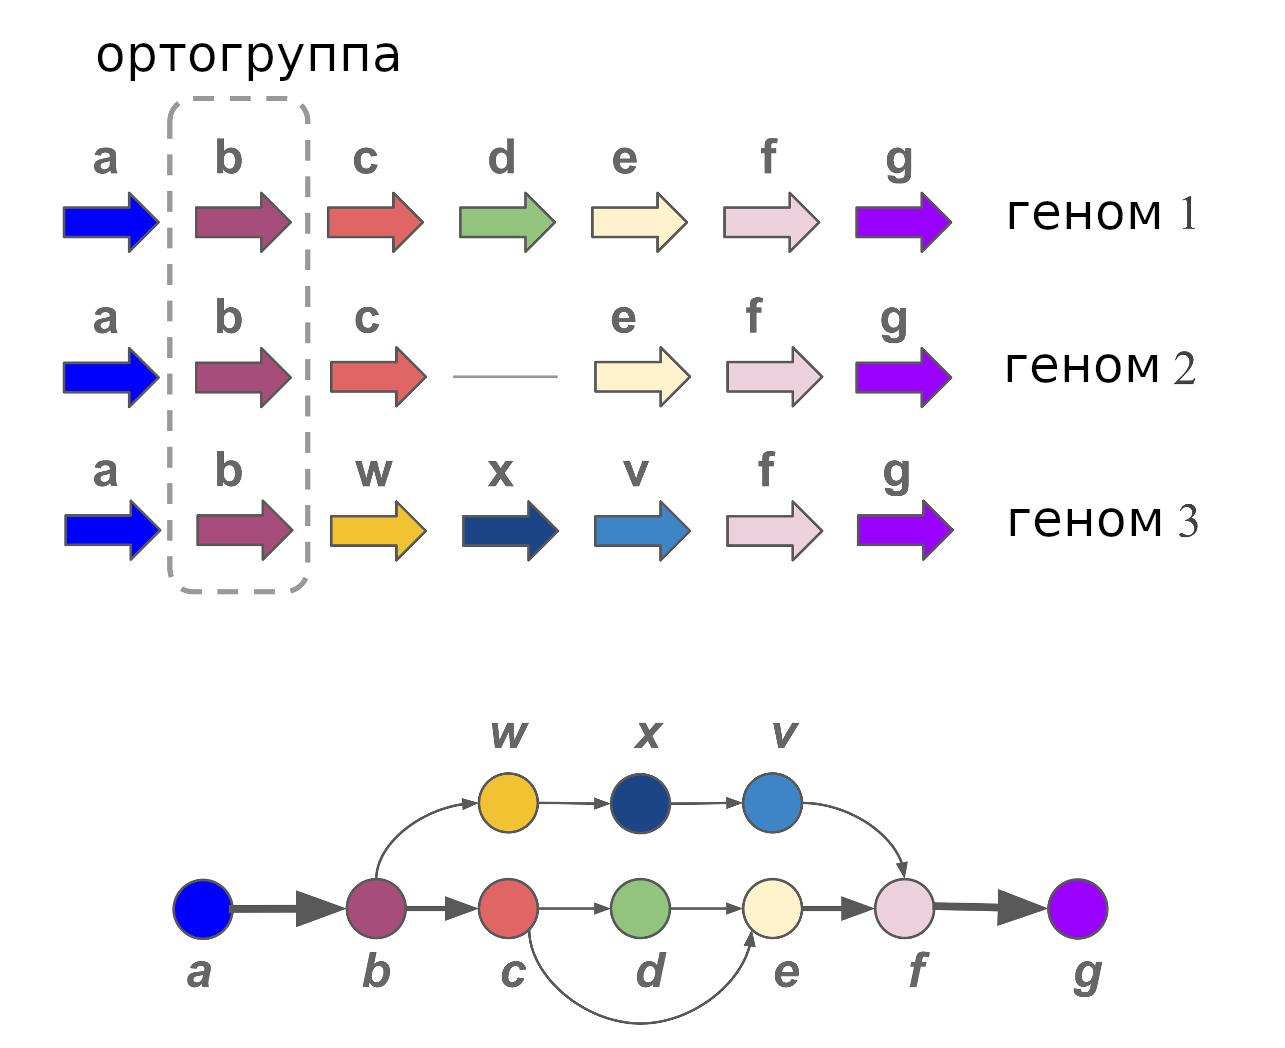
\includegraphics[width=0.8\textwidth]{Dissertation/images/graph/graph_scheme.png}
  \caption{Представление контекста генов в виде графа. Рассматриваем три гипотетеических генома, состоящих из 6-7 генов. Гены показаны стрелками, цветом и буквами обозначены гены, относящиеся к одной ортогруппе. В нижней части рисунка показано графовое представление для данного набора геномов.}
  \label{img:scheme} 
\end{figure}

Предложенная схема требует уточнения в случае, когда несколько генов из одной геномной последовательности принадлежат к одной ортогруппе (мы будем называть такие гены паралогами). Мы предложили два подхода представления паралогичных генов в графе. В первом случае мы игнорируем паралогичные гены и не добавляем их в граф. Во втором --- мы проводим процедуру "ортологизации"\ паралогичных генов: гены из ортогруппы добавляем в граф с некоторым суффиксом, при этом гены имеющие одинаковый контекст добавляются с одним и тем же суффиксом. В нашей программной реализации пользователь может выбирать применяемый подход. 

\subsection*{Оценка изменчивости геномов при помощи графового представления}
В качестве меры локальной изменчивости геномов мы предложили использовать подсчет количества путей в соответствующем подграфе. В случае, если в некотором регионе не происходит изменений генного состава, то подграф представляет из себя простую структуру с одним возможным путем (способом обхода узлов). В случае, если в данной области происходят изменения, то в подграфе появляются новые пути. Чем больше различных вариантов сочетания генов наблюдаются в геномных последовательностях, тем больше путей в соответствующем подграфе. 

Оценка локальной вариабельности производится для одного гена референсного генома с учетом окна (смежных генов), размер которого можно задавать при запуске алгоритма. Алгоритм рассчета состаит в следающем. Вначале строится референсная цепочка узлов, после чего происходит подсчет путей, которые огибают узел(начинаются по одну сторону, а заканчиваются -- по другую). Подсчет числа путей в графе --- сложная вычислительная задача, относящаяся к классу NP-полных (время решения экспоненциально зависит от размера графа). Поэтому мы выбрали вероятностный подход к подсчету числа путей. Мы задаем максимальное значение итераций и каждую итерацию ищем путь, начиная с первого узла референсной цепочки и затем выбирая следующие вершины случайным образом, пока путь не вернется в референсную цепочку, либо пока не будет достигнуто максмальное количество переходов. Количество найденных различающихся путей мы считаем мерой локальной изменчивости. Реализация метода доступна в пакете gene-graph-lib для языка Python.

\subsection*{Верификация метода оценки локальной изменчивости}
Для верификации предложенного алгоритма и его програмной реализации мы провели компьютерное моделирование эволюции геномов. Для каждого локуса моделируемого генома мы задавали опреленный уровень изменчивости, вероятностным образом измененяли генный состава и потом оценивали вариабельность при помощи предложенного нами подхода. Изменения генного состава происходили за счет вставки, удаления либо перемещения генов а также инверсий фрагментов генома. Вероятность инверсий была в 100 рез меньше вероятностей остальных событий, а размер области для инверсии выбирался случайно из экспоненциального распределения. Локализация событий изменений генного состава выбиралась случайно в соответствии с распределенией уровня вариабельности. Значения локальной вариабельности задавались в соответствии с одним из типов профилей: пилообразным, ступенчатым либо синусоидальным. Значения коэффициента $R^2$ были равны 0.95, 0.77 и 0.8 для ступенчатого, синусоидального и пилообразного профиля, соответственно. 


\subsection*{Анализ расположения областей повышенной изменчивости в геномных последовательностях кишечной палочки}
Для проведения данного анализа мы собрали коллекцию из 327 геномов бактерии \textit{E. coli} доступных в базе данных RefSeq, построили группы гомологии при помощи программы Orthofinder и применили разработанной нами метод оценки уровня геномной вариабельности, в качестве референсного генома был выбран геном штамма LF82, изолированного из пациента с болезнью Крона. На рисунке~\ref{img:complexity_lf82} показан профиль изменчивости и области расположения профагов, островов патогенности, генов рекомбиназ (для выявления следов мобильных элементов генома), жизненно необходимых генов (мутации в которых являются летальными) и генов транспортных и рибосомальная РНК.

\begin{figure}[!ht] 
    \center
      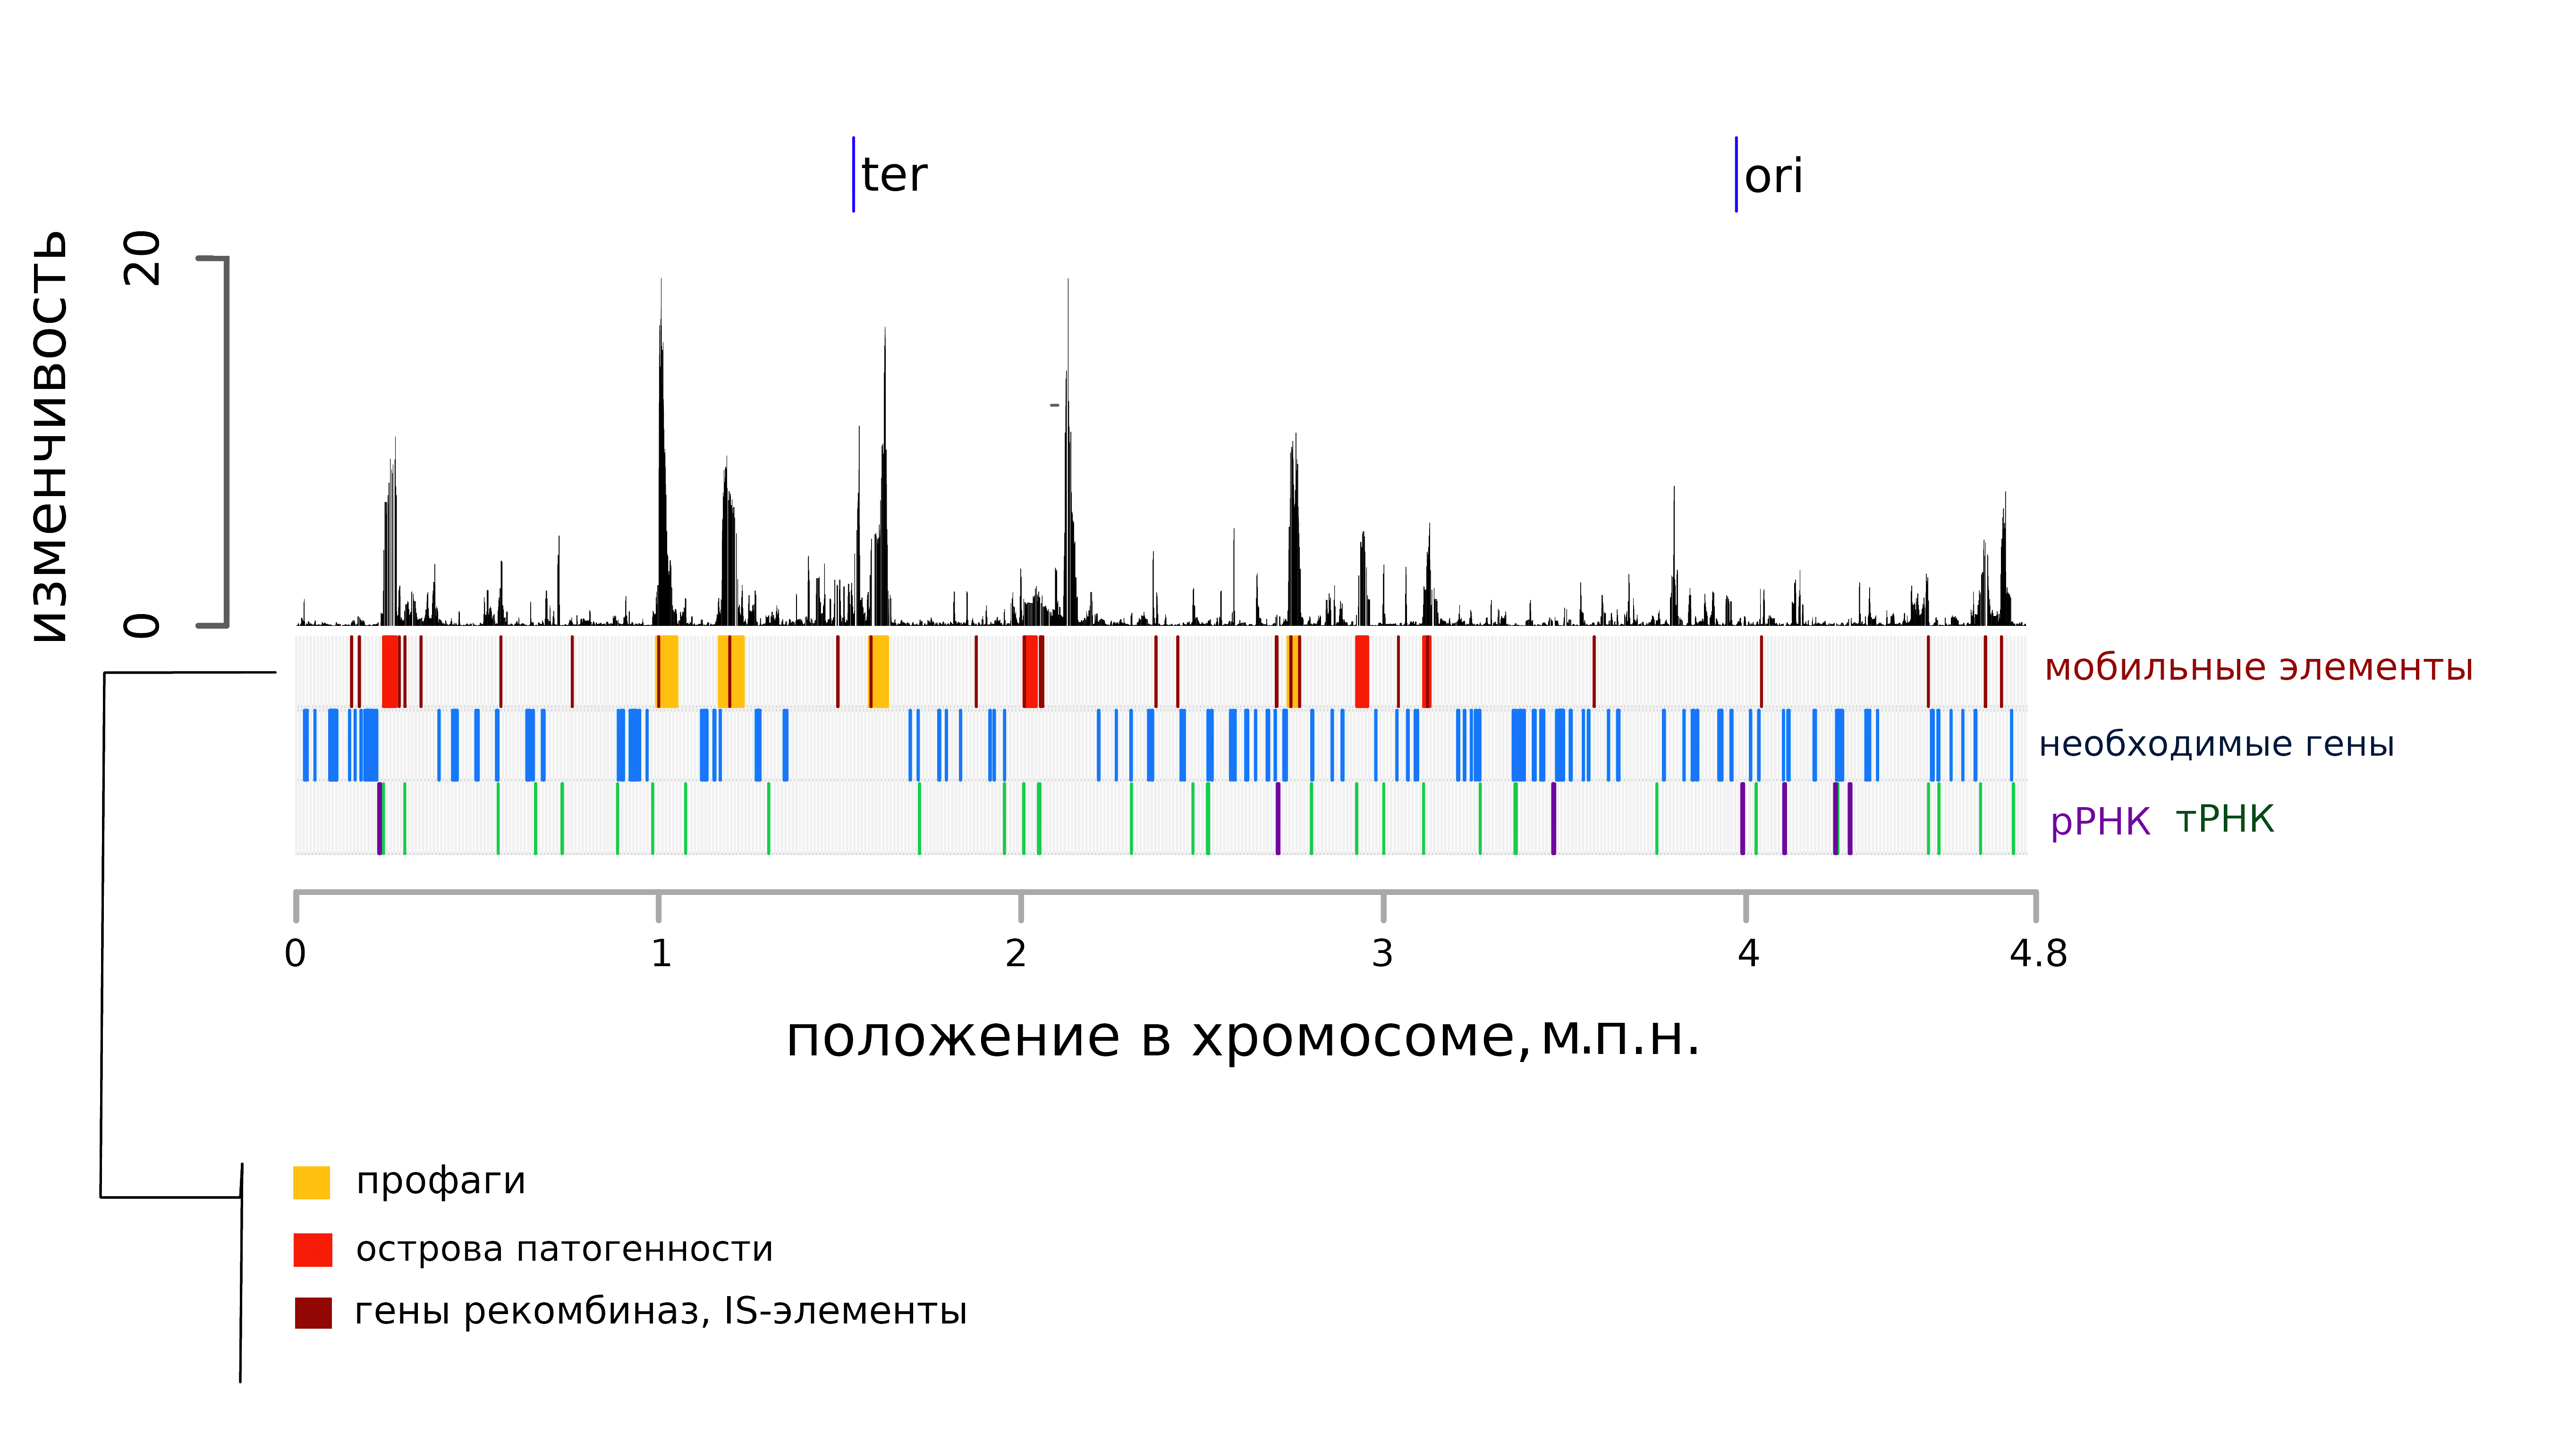
\includegraphics[width=\textwidth]{Dissertation/images/complexity/figure5plus.png}
    \caption{Профиль вариабельности генома \textit{Escherichia coli LF82}. Цветом обозначены острова патогенности, профаги,  гены, ассоциированные с мобильными элементами генома, жизненно-необходимые гены, гены транспортных и рибосомных РНК. Области повышенной изменчивости содержат меньше жизненно-необходимых генов. Профаги и острова патогенности обладают повышенным уровнем изменчивости по сравнению с остальной частью генома.}
    \label{img:complexity_lf82} 
  \end{figure}

Можно заметить, что участки генома в которых расположены жизненно необходимые гены, как правило, мало изменчивы а к высокоизминчивым областям генома относятся профаги и острова патогенности. При этом, наблюдаются также высокоизменчивые области генома, в которых отсутствуют признаки мобильных элементов; причины их высокой изменчивости остаются неизвестными. 

Гены транспортных РНК не проявлят явной ассоциации с профилем изменчивости. Гены рибосомальной РНК находятся преимущественно в мало изменчивых областях генома. 

Время существования вида \textit{Escherichia coli} оценивается в несколко десятков миллионов лет; возникает вопрос об устойчивости расположения горячих областей генома с течением времени. Для анализа этого вопроса мы провели сравнение профилей изменчивости подвидовых структур.  Для кишечной палочки существует устоявшаяся классификация клад филогенетического дерева, называемых филогруппами.  Для создания набора геномов мы выбрали по одному представителю из наиболее крупных филогрупп (A, B1, B2, E) и подобрали для каждого из них  по сто ближайший геномов из базы NCBI RefSeq. Затем мы рассчитали профили изменчивости для каждой филогруппы в отдельности и сравнили их между собой. Результат сравнения показан на рисунке~\ref{img:phylogroups_complex}, серым цветом обозначены блоки синтении, оранжевым -- области нахождения профагов.    

\begin{figure}[!ht] 
    \center
      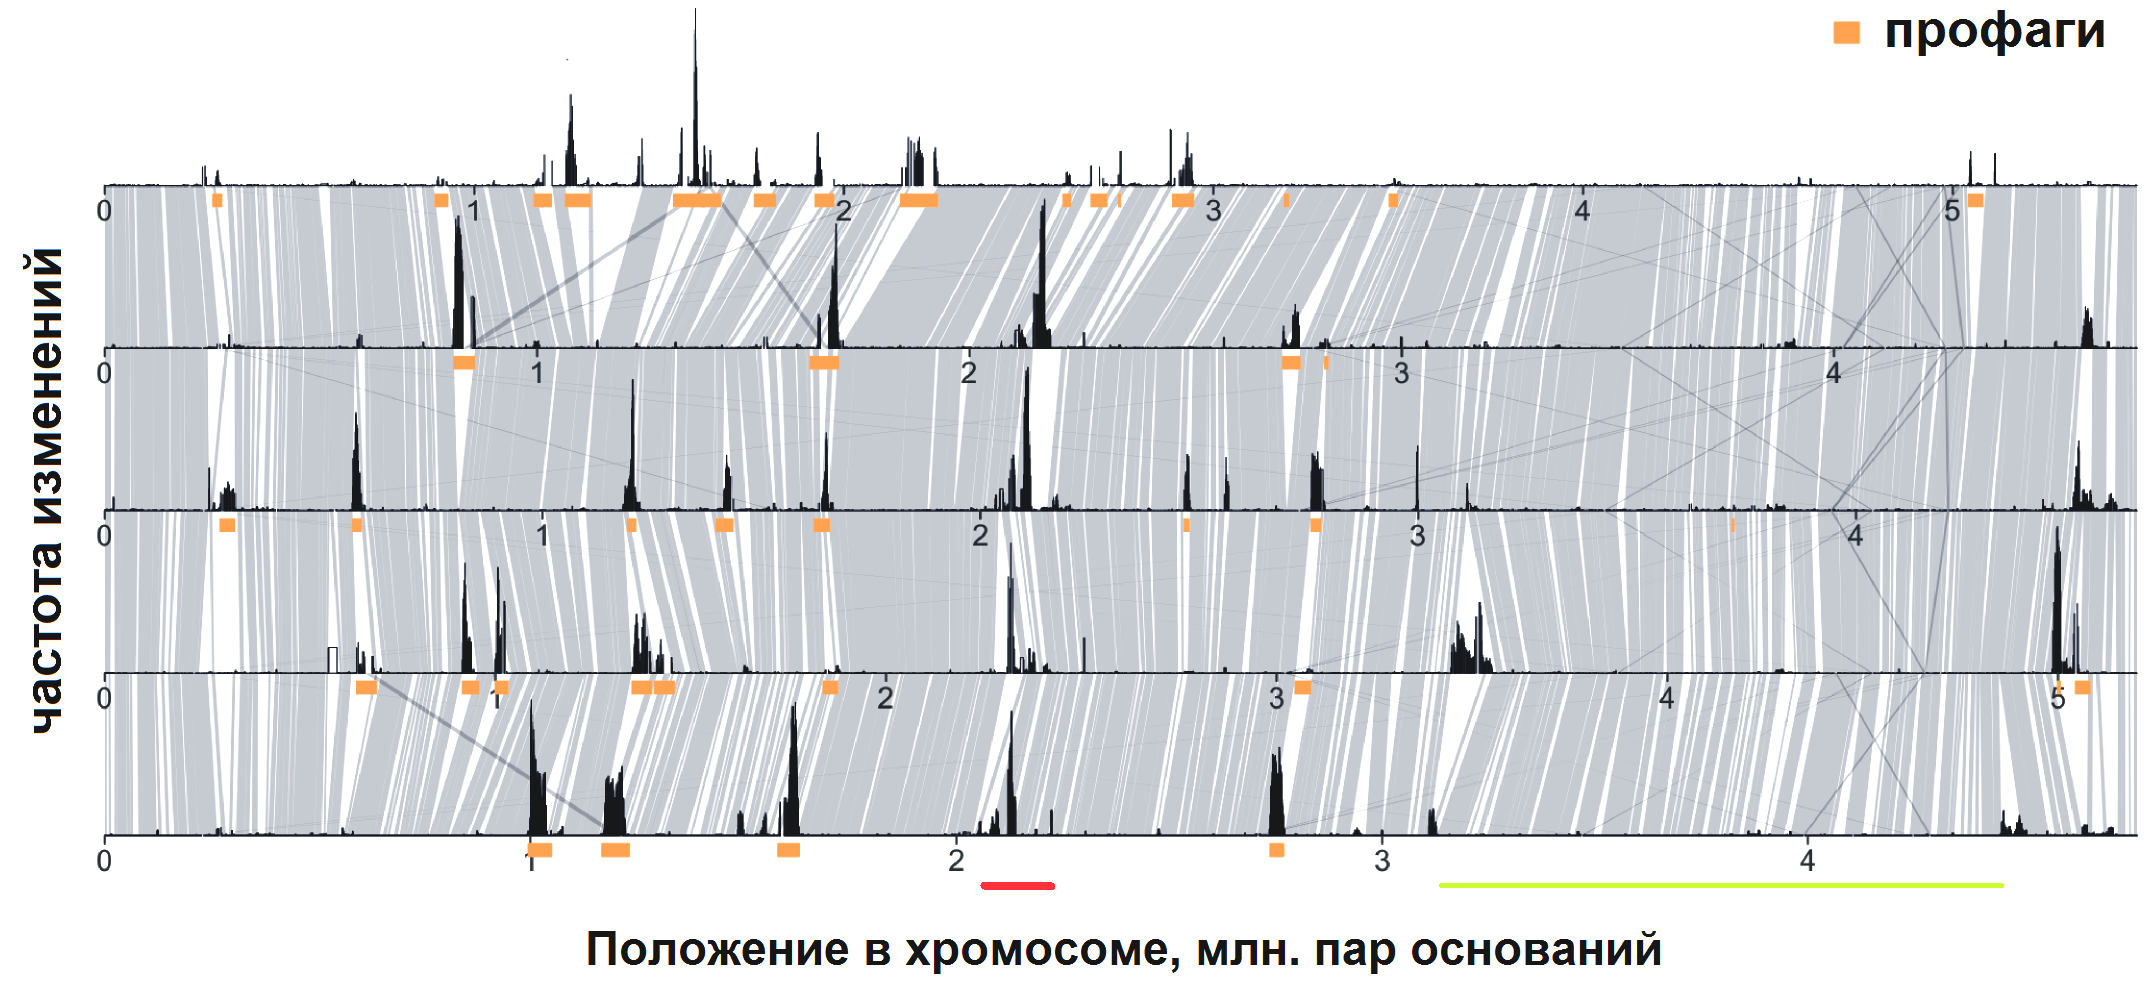
\includegraphics[width=\textwidth]{Dissertation/images/complexity/coli_phylogroups_complexity2.png}
    \caption{Сравнение профилей вариабельности представителей пяти филогрупп \textit{E. coli LF82}. Оранжевым цветом выделены области, определенные как профаговые. Блоками серого цвета показаны области синтении.}
    \label{img:phylogroups_complex} 
  \end{figure}
  

Сравнение показывает, что ряд областей генома с повышенной изменчивостью присутствуют во всех или в большинстве филогрупп, что, по-видимому, свидетельствует об их длительном существовании на протяжении значительной части времени жизни вида. Часть из этих областей соответствуют местам расположение профагов и их устойчивость можно объяснить сайт специфичным характером встраивания данных элементов. Одна из устойчивых горячих точек (выделена линией красного цвета) не имеет выявленных признаков мобильных элементов генома (рисунок~\ref{img:phylogroups_complex}). Значительная часть горячих областей геномов являются местами встройки фагов, что особенно заметно на примере филогруппы E, для которой была описана вирусная экспансия, значительно удлинившая их геномную последовательность (на рисунке длины геномов приведены к одинаковой ширине, но о размере генома можно судить по координатным осям ниже пролфилей изменчивости).

Заметно также существование и "холодных"\ областей генома с низкой вариабельностью во всех филогруппах. Длина этих маловариабельных участков может значительно превышать характерные длины оперонов, и достигать величин порядка миллиона пар оснований (например, область в окрестности 4 млн. п.н. на рисунке~\ref{img:phylogroups_complex}А, выделена линией зеленого цветом).

\subsection*{Разработка и применение графового подхода для визуализации локальной вариабельности геномов}

Множество сочетаний генов, которые наблюдаются в наборе геномов, можно представить в виде графа и использовать его для визуализации сравнений геномных последовательностей. Преимуществом данного подхода является компактность визуализации, так что становится возможным сравнение генных контекстов в сотнях геномных последовательностях. Компактность достигается за счет того, что консервативное сочетание генов (встречающиеся в большом количестве геномов) представлено на визуализации при помощи одного ребра, вне зависимости от количества геномов. Новые узлы и ребра добавляются в граф только в случае, когда ранее подобные сочетания не наблюдались. 

Визуализация полного графа для набора геномов возможна в случае небольших вирусных геномов; в случае бактериальных геномов имеет смысл проводить визуализацию и анализ подграфа --- части полного графа, соответствующей некоторому региону интереса (например, оперону).

Первым шагом алгоритма является построение \textit{референсной цепочки узлов} --- узлов графа, которые соответствуют генам референсного генома расположенным в выбранном регионе. Далее, в подграф включаются все пути, которые начинаются и заканчиваются на референсной цепочке. Мы предусмотрели несколько фильтров, позволяющих снизить количество отображаемымых узлов и ребер. Фильтр минимального веса ребра позволяет отсечь ребра, которые представляют редкие сочетания генов (встречающиеся в небольшом количестве геномов). Фильтр длинных путей заменяет слишком протяженные цепочки узлов (могут появиться в результате геномных перестроек) на короткие фрагменты ("хвосты"\ ) некоторой заданной длины. 

Визуализация подграфов обладает практической ценностью, поскольку позволяет создавать наглядную визуализацию возможных сочетаний генов в определенной области генома. Подобный тип визуализации можно использовать для определения того, представлен ли некоторый оперон в одном и том же генном контексте, или в разных. Под генным контекстом мы понимаем гены, расположеные непосресдвенно перед и после оперона. Мы говорим об одинаковом контексте в случае, если гены перед опероном относятся к одной ортогруппе, и гены после оперона относятся к некоторой другой ортогруппе; в графовом представлении, при этом, мы будем наблюдать, что цепочка узлов, соответствующая генам оперона, будет соединена с одним узлом с одной стороны и с другим узлом --- с другой. 


\subsection*{Примеры применения графового подхода для визуализации сравнения геномов}

В работе \cite{rakitina2017genome}, нами были установлены опероны, которые статистически значимо чаще встречались у изолятов \textit{E. coli} полученных от пациентов болезнью Крона (воспалительное заболевание кишечника), по отношению к изолятам от здоровых людей. Носительство данных оперонов, вероятно, выгодно при нахождении бактерий в условиях воспалительной реакции со стороны организма хозяина, а может и провоцирует воспаление. Метод для поиска оперонов, различающих группы бактерий, будет описан ниже.

Рассмотрим, как выглядят подграфы, соответствующие некоторым из выявленых оперонов. На этих примерах будут проиллюстрированы основные моменты анализа графового представления фрагментов генома. 

\textbf{Опероны утилизации гемина и пропандиола}

На рисунках~\ref{img:sub_hem} и ~\ref{img:sub_pdu} показаны графы, построенные в окрестностях оперонов захвата гемина (hemin uptake, hmu) и утилизации пропандиола (propanediol utilization operon, pdu), соответственно. В качестве референсного генома нами был взят геном \textit{Escherichia coli LF82}, в анализ были включены 327 финишированных геномов доступных в базе RefSeq. 

Рассмотрим для начала более простой случай оперона захвата гемина. Как видно из графа, представленного на рисунке~\ref{img:sub_hem}, данный оперон расположен в консервативном генном контексте. Дуговое ребро выходящее оперон сверху говорит о том, что в некотором наборе геномов данный оперон отсутствует и других последовательностей генов в этом локусе не наблюдается. 

\begin{figure}[!ht] 
  \center
  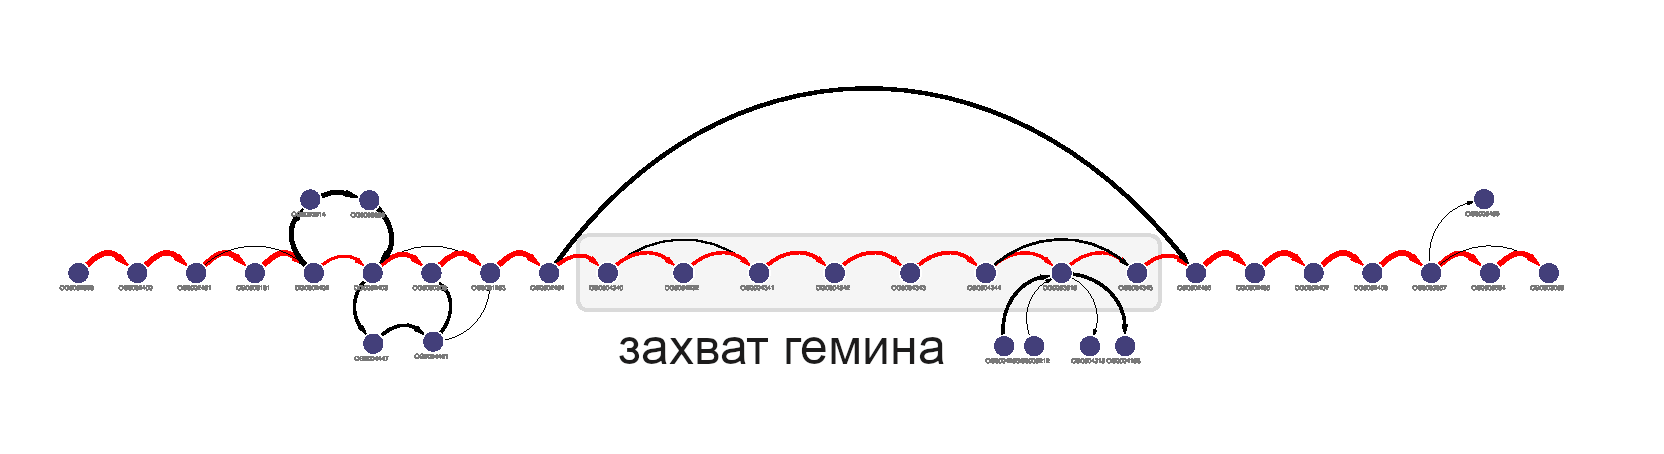
\includegraphics[width=0.8\textwidth]{Dissertation/images/subgraphs/hemin.png}
  \caption{Граф представляющий окрестность оперона утилизации гемина (hemin uptake, hmu). В ряде геномов оперон отсутствует, что видно из наличия ребра в графе, которое начинается перед и заканчивается непосредственно после генов оперона. }
  \label{img:sub_hem} 
\end{figure}

Для оперона утилизации пропандиола также наблюдается консервативность его рассположения. Ребро обходящее оперон (дуга ниже оперона) говорит о том, что в ряде штаммов в данном контексте нет иных вариантов последовательностей генов. Наблюдается некоторая вариабельность внутри оперона, соответствующая нескольким вариантам данного оперона \cite{rakitina2017genome}. Помимо pdu оперона, в том же контексте, у ряда штаммов наблюдается альтернативный набор последовательностей генов. В этот альтернативный набор входят гены транспорта железа (FepC, FcuA, HmuU), гены мобильных элементов (retroviral integrase core domain, transposase DDE Tnp ISL3) и множество гипотетических генов с неизвестной функцией. Примечательна вариабельность этого альтернативного набора генов. Вероятно, данный участок генома часто служит местом рекомбинационных событий, приводящих к изменению набора генов, причем эти изменения не имеют строгого начала и конца (т.е. не сайт специфичны), но часто накладываются друг на друга. 

\begin{figure}[!ht] 
  \center
    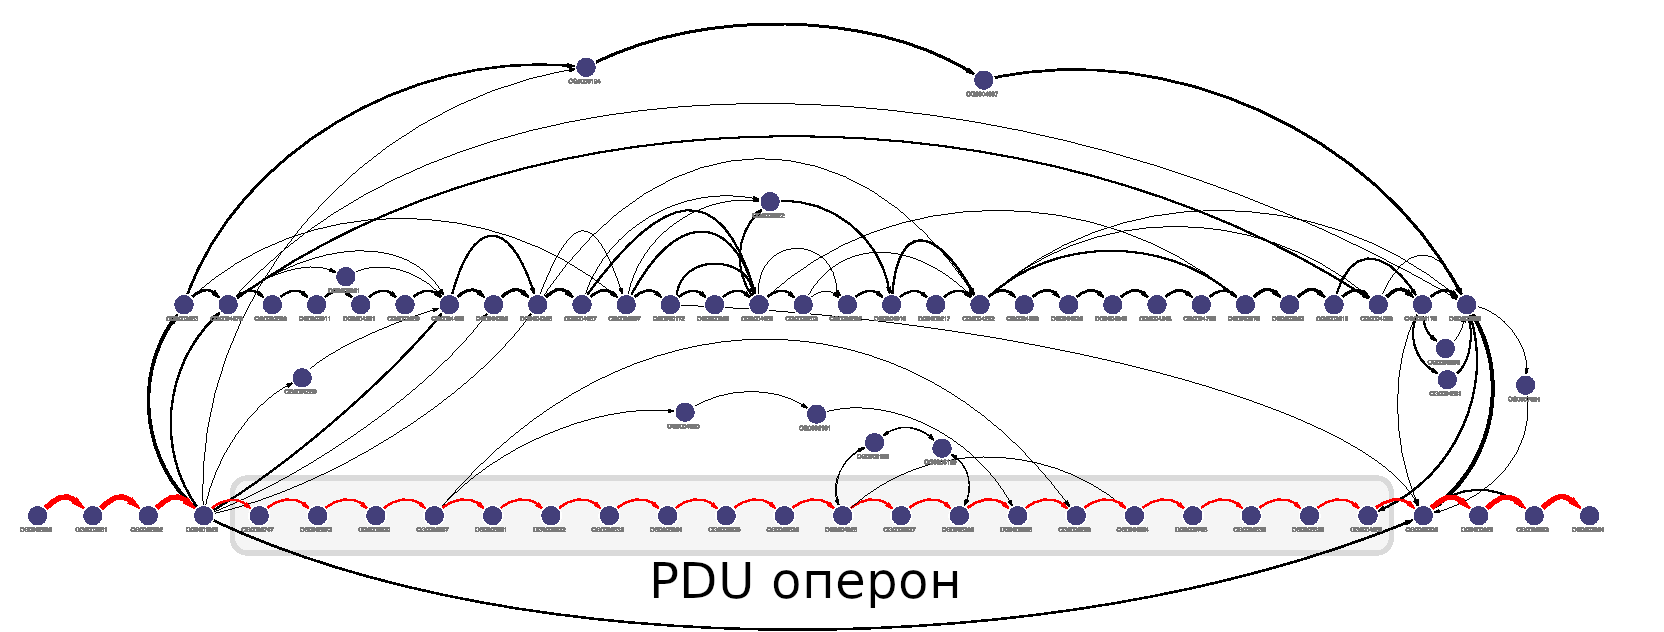
\includegraphics[width=0.8\textwidth]{Dissertation/images/subgraphs/pdu_laconic.png}
  \caption{Граф представляющий окрестность оперона утилизации пропандиола (propanediol utilization operon, pdu). Видна значительная вариабельность генного состава в данном регионе, что отражено во множестве путей на графе обходящих область генов оперона.}
  \label{img:sub_pdu} 
\end{figure}

\textbf{Кластер генов синтеза бактериальной капсулы}

Перейдем к описанию графа, представляющего окружение оперона синтеза капсулы, также чаще встречающегося у изолятов из пациентов с болезнью Крона. На рисунке~\ref{img:capsule_sub_small} показано ближайшее окружение данного оперона, сам оперон обведен рамкой серого цвета. 

\begin{figure}[!ht] 
  \center
    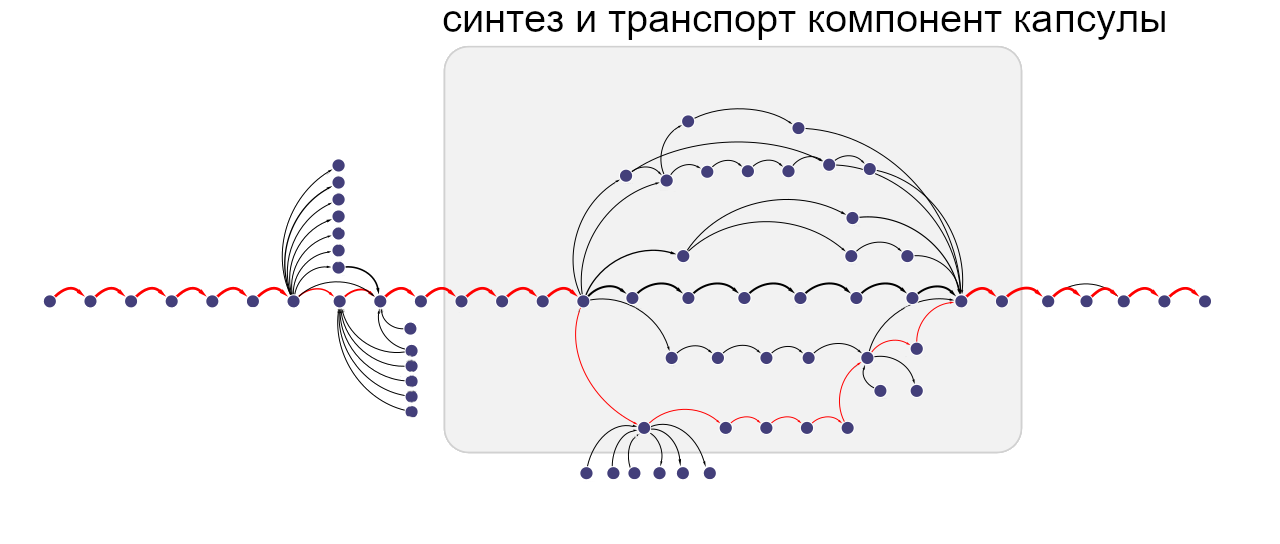
\includegraphics[width=\textwidth]{Dissertation/images/subgraphs/capsular_subgraph.png}
  \caption{Граф представляющий окрестность кластера генов синтеза бактериальной капсулы. }
  \label{img:capsule_sub_small} 
\end{figure}

Видно, что оперон состоит из консервативных фрагментов, окружающих вариабельный участок. Вариабельная часть оперона соответствует генам, отвечающим за синтез серотип-специфичного набора полимеров капсулы; гены консервативной части кодируют белки, участвующие в транспорте синтезированных веществ через клеточную стенку.

Таким образом, предложенный нами способ визуализации позволяет определить общую вариабельность генного состава в определенном локусе генома, выявить встречающиеся варианты взаимного расположения генов и, в частности, выявить вариабельный и консервативные области оперонов.

\subsection*{Разработка компьютерного приложения для анализа вариабельности геномов} \label{chaptGCB}

Оценка профиля изменчивости вдоль хромосомы и визуализация подграфов для отдельных локусов --- это варианты анализа геномной изменчивости, которые позволяют проводить анализ на уровне отдельных репликонов в первом случае, и на уровне небольших геномных локусов (например, оперонов) --- во втором. Для проведения анализа на двух уровнях одновременно мы разработали приложение Genome Complexity Browser (GCB). Данное приложение доступно по адресу \url{gcb.rcpcm.org}, и может быть запущенго на локальном компьютере пользователя. Веб-версия содержит данные о геномной изменчивости для 143 видов прокариот. Использование локальной версии необходимо при анализа групп геномов не представленных на веб-сервере.

Основные сценарии использования программы следующие:

I. Если интерес представляет некоторый оперон или группа генов.

Пользователь выбирает организм, геном и задает координаты области интереса. Происходит построение подграфа для выбранной области. При необходимости, пользователь меняет параметры визуализации (например, увеличивает минимальный отображаемый вес ребра для исключения редко встречающихся комбинаций генов, в случае если получаемый граф слишком сложен для анализа). Экспорт полученной визуализации в графическом формате, либо в формате XML для последующей визуализации подграфа в программе Cytoscape (графовый редактор). 

II. Если интерес представляют области повышенной либо пониженной изменчивости генома.

Пользователь выбирает организм и геном. Происходит визуализация профиля изменчивости выбранного генома. Пользователь может выбрать интересующий его регион генома (например, область с максимальным уровнем изменчивости) и выполнить визуализацию подграфа в данной области - таким образом можно установить, какие гены содержатся в данном локусе у различных геномов, и каков паттерн зафиксированных в ходе эволюции изменений. Пользователь может экспортировать профиль изменчивости в виде текстового файла, для последующей визуализации (например, сравнение профилей изменчивости разных организмов), либо сохранить области с повышенной изменчивостью в файл в формате BED. 

\textbf{Возможности программы}

В программе предусмотрено автоматическое выделение "горячих точек" изменчивости. Они отображаются на профиле изменчивости (точки оранжевого цвета, расположенные ниже профиля), и их положение можно скачать в виде файла в формате BED. Для выделения областей повышенной изменчивости, мы использовали критерий Тьюки: искали значения уровня вариабельности, которые превышают 75 перцентиль на полтора межквартильных расстояния. 

Для анализа геномов, недоступных на веб-сервере, необходимо использование локальной версии программы. Схема анализа показана на рисунке~\ref{img:gcb_scheme}.

\begin{figure}[!ht] 
	\center
	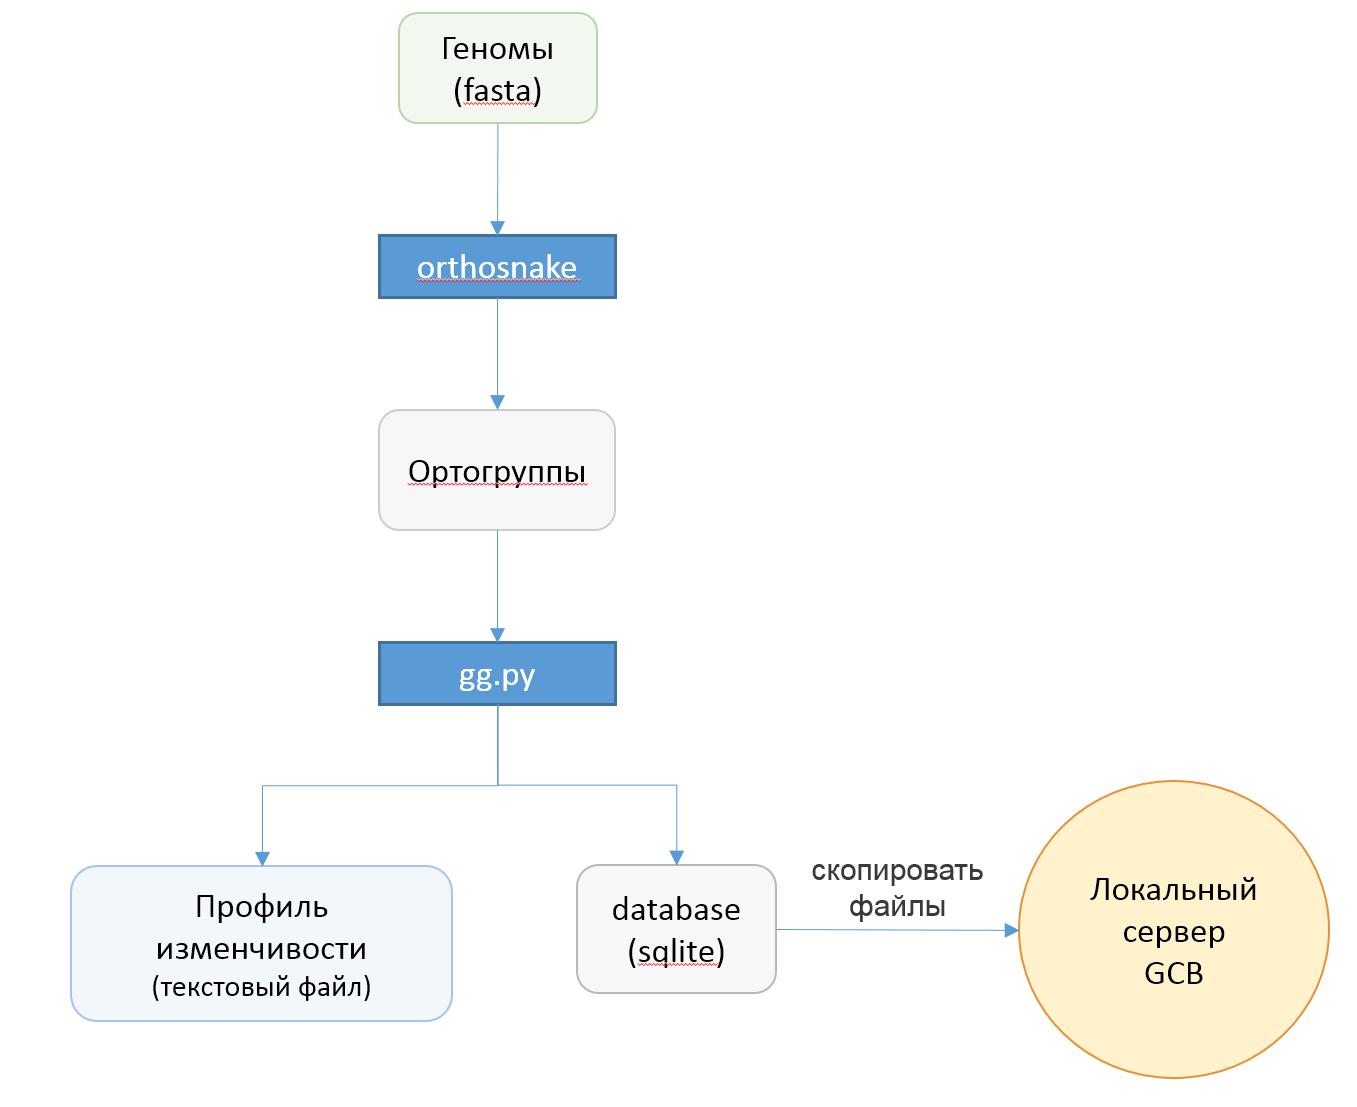
\includegraphics [width=0.9\textwidth] {Dissertation/images/gcb/standalone_scheme.png}
	\caption{Схема обработки геномных последовательностей для анализа их вариабельности.}
	\label{img:gcb_scheme}
\end{figure}

Документация и видеоматериалы по использованию программы (как веб-версии, так и консольных утилит) доступны по адресу \url{gcb.readthedocs.io}. 

\subsection*{Алгоритмизация подхода выявления оперонов, наличие которых ассоциировано с определенным признаком. } \label{chaptOperons}

Предположим, что у нас есть некоторый признак, по которому мы можем разбить набор геномов на группы, и наша задача --- установить, какие гены значимо чаще (либо реже) встречаются в одной из групп. Простым и распространенным методом анализа, в подобном случае, является вычисление статистики и оценка значимости по каждому отдельному гену. После проведения этих тестов необходимо применить поправку на множественное сравнение, так как иначе следует ожидать множество ложно положительных результатов. В случае, если работа ведется на данных о полной последовательности генома, имеется большое количество анализируемых генов (порядка $10^3 - 10^4$), а размеры групп, как правило, незначительны (порядка $10^1 - 10^2$), что приводит к тому, что после поправки на множественное сравнение, ни один из анализируемых генов не проходит даже низкие пороги на значимость. В качестве одного из способов преодоления описанной выше проблемы мы предложили использовать информацию об организации генов в опероны для поиска значимых ассоциаций \cite{rakitina2017genome}. Рассматривая оперон как структурную единицу, мы значительно сокращаем количество анализируемых признаков.

\textbf{Алгоритм поиска генетических ассоциаций}
На входе необходимо иметь два или более набора геномных последовательностей, различающихся по некоторому признаку (например, наличию заболевания у организма-хозяина), также необходимо выбрать один референсный геном для которого известно расположение оперонов в геномной последовательности.

Первым шагом выполняется построение групп гомологий и оценка статистической значимости их неравной представленности в сравниваемых выборках. Таким образом мы получаем набор генов, ассоциированных с некоторым признаком. Затем ищутся опероны, в которых количество найденных ассоциированных генов выше, чем ожидалось бы при случайном распределении генов по оперонам. Для оценки ожидаемого количества генов при их случайном распределении по оперонам мы предложили использовать два подхода. Первый основан на пермутациях таблицы соответствий генов и оперонов, выполняемой 10000 раз. Второй предполагает рассчет ожидаемого значения исходя из расспределения Пуассона, параметр которого рассчитывается как доля значимо ассоциированных генов среди общего числа генов в референсном геноме. Финальным шагом является проведение поправки на множественное сравнение, но уже не для генов, а для оперонов, количество которых, как правило, значительно ниже общего количества генов. 

\textbf{Поиск оперонов, значимо чаще встречающихся у изолятов бактерий \textit{E. coli}, изолированных от людей с болезнью Крона}
В анализе были использованы геномные последовательности 51 изолятов \textit{E. coli}, 27 из которых были получены от пациентов с болезнью Крона, а 24 --- от здоровых людей. При помощи программы OrthoFinder мы получили 11885 групп гомологии. Далее, при помощи точного теста Фишера оценили статистическую значимость их неравномерной представленности.  

Следующим шагом мы осуществили описанный выше тип анализа, для поиска значимо дифференциально представленных оперонов. Информация об оперонах была взята из базы данных DOORS. В качестве референсного генома мы использовали геном \textit{Escherichia coli LF82} - данный штамм был изолирован из пациента с болезнью Крона и является модельным в исследованиях адгезивно-инвазивного фенотипа у кишечной палочки. Затем, мы провели 10000 случайных перестановок соответствий между генами и оперонами. Для каждой перестановки мы вычисляли зависимость количества генов в оперонах с p-value < 0.05 от длины оперона. Визуализация сравнения наблюдаемых и полученных при случайных перестановках результатов показана на рисунке~\ref{img:operons_shuffle}. Опероны, для которых наблюдаемое число генов было выше, чем максимальное количество генов при случайных перестановках, считались статистически значимо пере- либо недо-представленными, поскольку для них можно считать, что в пермутационном тесте p-value < 0.0001. 

\begin{figure}[!ht] 
  \center
    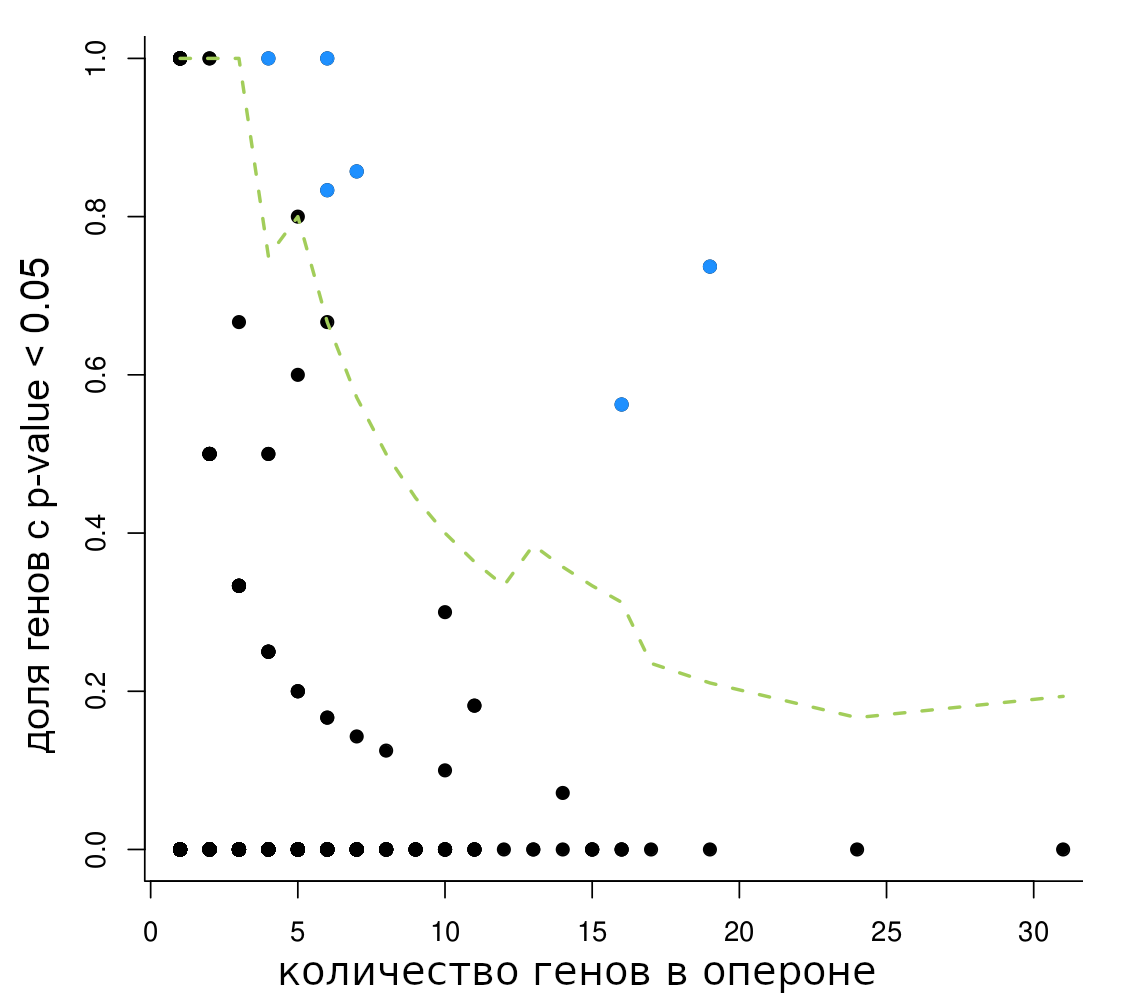
\includegraphics [width=0.75\textwidth] {Dissertation/images/operons/statsignificant_operons.png}
    \caption{Зависимость доли генов в оперонах, с уровнем значимости p-value < 0.05, от количества генов входящих в оперон. Пунктирная линия показывает максимальные значения, полученные при проведении 10000 случайных соотнесений генов и оперонов.}
    \label{img:operons_shuffle}
\end{figure}

Так, например, оперон утилизации пропандиола состоит из 19 генов, из которых 14 генов (74\%) имеют p-value < 0.05 в точном тесте Фишера. При проведении 10000 случайных пермутаций уровней значимости по генам, в данном опероне в среднем наблюдалось 3\% генов, а максимальная доля составила 21\%. Таким образом, можно сделать вывод, что повышенная представленность данного оперона в изолятах из пациентов, но не здоровых людей, не является случайным наблюдением. Полный список оперонов, определенных как значимо чаще встречающихся у изолятов из пациентов с болезнью Крона приведен в таблице~\ref{tbl:ops1}. 

\begin{table}[htbp]
\centering
\caption{Список оперонов статистически значимо пере-представленных в группе штаммов \textit{E. coli} изолированных из пациентов с болезнью Крона. N - количество генов, Pobs - наблюдаемое количество пере-представленных генов в опероне, Pmean - среднее количество перепредставленных генов при случайных пермутациях, Pmax - максимальное количество перепредставленных генов при случайных пермутациях.}
\label{tbl:ops1}
\begin{tabular}{|l|l|l|l|l|}
\hline
\textbf{N} & \textbf{Pobs} & \textbf{Pmean} & \textbf{Pmax} & \textbf{функция}                                  \\ \hline
4          & 1             & 0.03          & 0.75         & glyoxilate metabolism operon \\ \hline
6          & 0.83          & 0.02          & 0.67         & capsular assembly PAI IV LF82                              \\ \hline
6          & 1             & 0.02          & 0.67         & hemin uptake operon                                       \\ \hline
7          & 0.86          & 0.03          & 0.57         & sorbose uptake and utilization                             \\ \hline
16         & 0.56          & 0.02          & 0.31         & prophage I LF82                                            \\ \hline
19         & 0.74          & 0.03          & 0.21         & propanediol utilization operon                         \\ \hline
\end{tabular}
\end{table}


\FloatBarrier
\pdfbookmark{Заключение}{conclusion}                                  % Закладка pdf
\section*{Заключение}

В нашей работе, мы использовали представление набора геномов в виде графа для двух задач: численной оценки уровня изменчивости в отдельных локусах генома и визуализации подграфов, соответствующих отдельным областям генома. Визуализация подграфов позволяет дать ответы на ряд вопросов о контексте генов интереса. Например, находится ли ген или гены интереса в одинаковом окружении во всех рассматриваемых геномах? Какие альтернативные генные контексты существуют и в каких геномах они представлены? Какие части набора генов (например, оперона или генного острова) являются консервативными, а какие вариабельными? Какие геномы содержат определенную комбинацию генов? 

При помощи графового представления геномов мы реализовали метод количественной оценки локальной изменчивости, основанный на поиске уникальных путей в подграфе. Под изменчивостью в данном случае мы понимаем изменение состава либо взаимного расположения генов в геноме. Под локальностью --- то, что изменения затрагивают небольшую область генома, не превышающую размер выбранного окна анализа (выбирается пользователем, обычно, составляет около 20-40 генов). Насколько нам известно, разработанный нами вычислительный конвейер (Genome Complexity Browser, GCB) является первым доступным инструментом, позволящим количественно определять изменчивость генома на основе заданного пользователем набора геномов. GCB предоставляет способ оценки профиля изменчивости вдоль репликонов, что позволяет находить "горячие точки"\ генома, в которых уровень изменчивости значительно выше, чем в остальной части генома, и его "тихие"\ области. Значительная часть высокоизменчивых областей генома соответствует местам встройки профагой и остравов патогенности. При этом, для кишечной палочки мы также наблюдали существование протяженной выосокоизменчивой области генома, в которой нет признаков наличия мобильных элементов. При этом данная область обладает высоким уровнем изменчивости у всех крупных филогрупп данного вида. 

Мы провели поиск оперонов, которые чаще встречаются у кишечных палочек, выделенных из образцов фекалий и кишечных смывов пациентов с болезнью Крона - тяжелого воспалительного заболевания кишечника. Функция большинства найденных оперонов ясна, они позволяют захватывать железо, утилизировать пропандиол (продукт переработки слизистого слоя), менять антигенные свойства, тем самым убегая от иммунного ответа. Интересно, что анализ графов, представляющих контекст этих генов, показал очень разные картины. Два оперона: утилизации пропандиола и производства капсулы находятся в высоко-изменчивых --"горячих"\ -- областях генома. Опероны утилизации гимина, утилизации глиоксилата, захвата сорбозы напротив находятся в "тихих"\ областях. Роль генетических факторов, находящихся в областях генома с разным уровнем изменчивости, в формировании генотипа и фенотипа бактерий --- предмет дальнейших исследований. В случае оперона синтеза и экспорта капсульных полисахаридов, можно предположить, что нахождение данного оперона в "горячей"\ области генома может способствовать более высокой изменчивости состава оперона (у него есть высоко вариативная часть, отвечающая за синтез капсулы), что в свою очередь выгодно для эффективного избегания иммунного ответа организма-хозяина.

\section*{Выводы}
\begin{enumerate}
\item Предложенный и реализованный в нашей работе способ графового представления расположения генов в наборе геномов является эффективным средством для визуального анализа изменений геномных изменений и поиска областей генома с повышенной изменчивостью, в том числе не несущих признаков мобильных элементов генома.

\item Геномы из различных филогрупп и филогенетически близких видов обладают как консервативными (расположенными в схожих местах генома), так и вариативными (присутствующими лишь у некоторых представителей) областями повышенной изменчивости.

\item Наибольшее количество областей повышенной изменчивости в рассмотренных геномах находится в областях локализации профагов.

\item Опероны, значимо чаще встречающиеся в изолятах \textit{E. coli}, изолированных от пациентов с болезнью Крона по сравнению с изолятами полученными от здоровых людей, расположены как в низко-изменчивых областях генома(опероны захвата сорбозы, захвата гимина, утилизации глиоксилата), так и в высокоизменчивых областях (оперон утилизации пропандиола, синтеза и экспорта капсульных полисахаридов).
\end{enumerate}

\pdfbookmark{Литература}{bibliography}                                % Закладка pdf


\ifdefmacro{\microtypesetup}{\microtypesetup{protrusion=false}}{} % не рекомендуется применять пакет микротипографики к автоматически генерируемому списку литературы
\urlstyle{rm}                               % ссылки URL обычным шрифтом
\ifnumequal{\value{bibliosel}}{0}{% Встроенная реализация с загрузкой файла через движок bibtex8
    \renewcommand{\bibname}{\large \bibtitleauthor}
    \nocite{*}
    \insertbiblioauthor           % Подключаем Bib-базы
    %\insertbiblioexternal   % !!! bibtex не умеет работать с несколькими библиографиями !!!
}{% Реализация пакетом biblatex через движок biber
    % Цитирования.
    %  * Порядок перечисления определяет порядок в библиографии (только внутри подраздела, если `\insertbiblioauthorgrouped`).
    %  * Если не соблюдать порядок "как для \printbibliography", нумерация в `\insertbiblioauthor` будет кривой.
    %  * Если цитировать каждый источник отдельной командой --- найти некоторые ошибки будет проще.
    %
    %% authorvak
    \nocite{tyakht2018genetic}
    \nocite{terekhov2018ultrahigh}
    \nocite{bulaev2017genome}a
    \nocite{zakharzhevskaya2017outer}
    \nocite{conf1}
    \nocite{conf2}
    \nocite{conf3}
    \nocite{novosibconf}
    \nocite{biotechconf2}
    \nocite{novosibconf}
    \nocite{pstutconf}
    \nocite{crohnconf}
    \nocite{crohnconf1}
    
   

    \ifnumgreater{\value{usefootcite}}{0}{
        \begin{refcontext}[labelprefix={}]
            \ifnum \value{bibgrouped}>0
                \insertbiblioauthorgrouped    % Вывод всех работ автора, сгруппированных по источникам
            \else
                \insertbiblioauthor      % Вывод всех работ автора
            \fi
        \end{refcontext}
    }{
        \ifnum \totvalue{citeexternal}>0
            \begin{refcontext}[labelprefix=A]
                \ifnum \value{bibgrouped}>0
                    \insertbiblioauthorgrouped    % Вывод всех работ автора, сгруппированных по источникам
                \else
                    \insertbiblioauthor      % Вывод всех работ автора
                \fi
            \end{refcontext}
        \else
            \ifnum \value{bibgrouped}>0
                \insertbiblioauthorgrouped    % Вывод всех работ автора, сгруппированных по источникам
            \else
                \insertbiblioauthor      % Вывод всех работ автора
            \fi
        \fi
        %  \insertbiblioauthorimportant  % Вывод наиболее значимых работ автора (определяется в файле characteristic во второй section)
        \begin{refcontext}[labelprefix={}]
            \insertbiblioexternal            % Вывод списка литературы, на которую ссылались в тексте автореферата
        \end{refcontext}
        % Невидимый библиографический список для подсчёта количества внешних публикаций
        % Используется, чтобы убрать приставку "А" у работ автора, если в автореферате нет
        % цитирований внешних источников.
        \printbibliography[heading=nobibheading, section=0, env=countexternal, keyword=biblioexternal, resetnumbers=true]%
    }
}
\ifdefmacro{\microtypesetup}{\microtypesetup{protrusion=true}}{}
\urlstyle{tt}                               % возвращаем установки шрифта ссылок URL
